\section{Initial Asteroid Results}
\label{sec:samples}

\subsection{The associated known-object population}
\label{sec:known_population}

The primary $1\asec$ sample contains 531,612 associations to
58,281 catalog identities on 128 physical observing nights.
Figure~\ref{fig:orbits} shows the cataloged orbital elements once
per identity, together with the number of observing nights and
the first-to-last measurement span. Counting identities once
separates the population represented in the catalog from the
detection-weighted sky map in Figure~\ref{fig:coverage}.

The adopted main-belt region contains 55,791 identities,
or 95.73\% of the sample. Other points occupy the inner-belt,
Mars-crossing, outer-belt, Jupiter Trojan, near-Earth, and
distant-orbit regions. Here the near-Earth label uses
$q<1.3$~au, while the distant label uses the broad cut
$a\geq5.4$~au. The Jupiter Trojan label denotes a
semimajor-axis region, not a resonance classification
derived in this work.

We examine the 119 positional associations to 17 catalog identities
in the distant-orbit region using neighboring exposures and local
image cutouts. Comparing a stationary-source hypothesis with the
predicted displacement supports motion for 79 associations belonging
to seven identities and identifies nine stationary-source
coincidences belonging to seven other identities. The remaining
31 associations lack sufficient local evidence: 28 belong to
identities supported by other measurements, while three are the
sole associations of three unresolved identities.
Figure~\ref{fig:orbits} retains the original positional-association
selection; the supplementary tables record the local evidence for
each identity and individual association.

The median identity has four associations on two
observing nights. The 75th percentiles are 13 associations
and six nights, respectively, and the maximum number
of distinct nights is 25. The median first-to-last
measurement span over all identities is 8.10~days.
Figure~\ref{fig:orbits}d emphasizes the longer baselines
of objects observed on multiple nights. These distributions
show the temporal information available for assembling
asteroid photometric and astrometric series, while also
showing that many identities have only sparse coverage.

\begin{figure}[tbp]
\centering
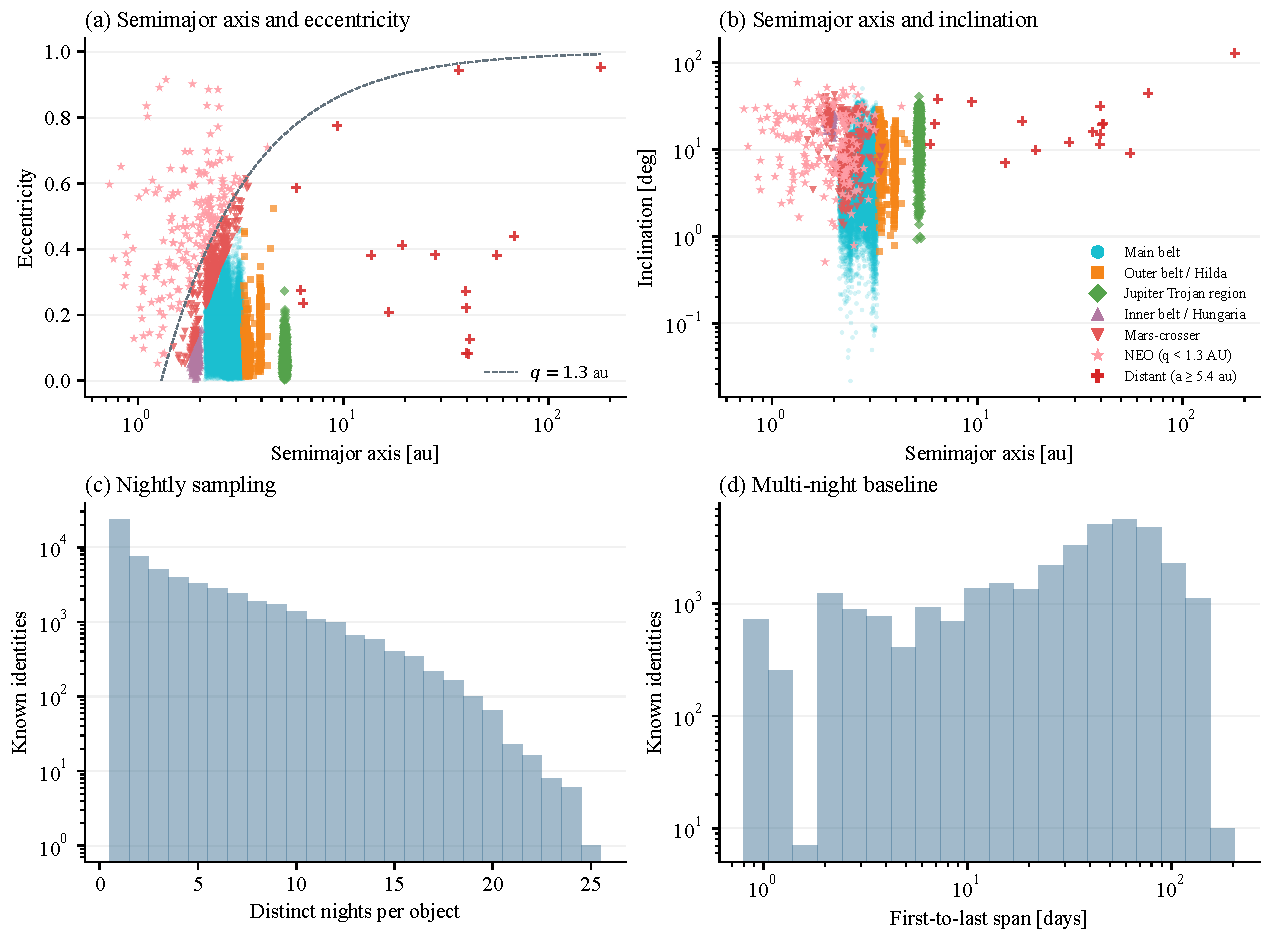
\includegraphics[width=0.98\linewidth]{fig07_orbits_and_revisits.pdf}
\caption{The associated known-object sample, counted once
per catalog identity. (a,b) Archived catalog semimajor
axis versus eccentricity and inclination. Colors and
symbols mark the adopted orbital regions; the dashed
curve in (a) is $q=1.3$~au. The Jupiter Trojan region
is a semimajor-axis selection. Distant-region points retain the 17 catalog identities in the
positional-association sample. Local checks support motion for seven
identities, identify stationary-source coincidences for seven, and leave
three without sufficient evidence.
(c) Number of distinct physical observing nights per
identity. (d) First-to-last measurement span for the
multi-night subset. The vertical count scales in
(c,d) and the semimajor-axis scales in (a,b) are
logarithmic.}
\label{fig:orbits}
\end{figure}

The viewing geometry is predominantly at large solar
elongation. Using target and solar directions from the
same observatory origin, the detection-weighted median
elongation of the validated association sample is
$149.34^\circ$, and its minimum is $59.72^\circ$.
The median measured angular rate of adjacent
within-night association pairs is
26.84~\rateunit. The calculation and distributions
are given in Appendix~\ref{app:checks}. The known-object
branch does not apply the independent search's
$3$--$63$~\rateunit\ window and therefore also records
faster known objects.

\subsection{Historical single-night candidates}
\label{sec:candidates}

The historical independent search produced 4,762
automatic single-night links. Their 14,299 membership
rows correspond to 14,159 unique detection keys because
a detection can occur in more than one proposed link.
Visual review initially marked 68 links as real; 67
were selected for submission, and subsequent image
review retained 58 links containing 179 measurements
on 34 nights (Table~\ref{tab:candidates}). All 179 measurements
map to validated exposures, and every retained linkage contains at
least three distinct exposures within one physical observing night.
The reviewed sample is therefore unchanged by exposure validation;
the automatic catalog and review stages retain the selection of
the original search.

\begin{table}[tbp]
\centering
\caption{Historical Single-Night Candidate Record}
\label{tab:candidates}
\begin{tabular}{lr}
\toprule
Stage & Number of links\\
\midrule
Automatic catalog & 4,762\\
Initially marked real in image review & 68\\
Selected for submission & 67\\
Retained after subsequent image review & 58\\
\quad Consistent with C/2025~Y1 in ephemeris checks & 6\\
\quad Identity unresolved in the frozen analysis & 52\\
\bottomrule
\end{tabular}
\tablecomments{The retained sample comprises 179
measurements on 34 nights, all in validated exposures. Links are single-night
measurement groupings; the entries are not counts
of independently identified new objects.}
\end{table}

Figure~\ref{fig:candidate} presents a retained
three-image sequence from 2026 February~10. The
midpoint times span approximately 79~min, and the
measured linear sky-plane rate is
61.34~\rateunit, close to the upper edge of the
historical search window. The sequence illustrates
the direct image evidence behind an individual
linkage. Appendix~\ref{app:shortarc} shows the arc
spans and short-arc residuals for the retained
sample.

\begin{figure}[tbp]
\centering
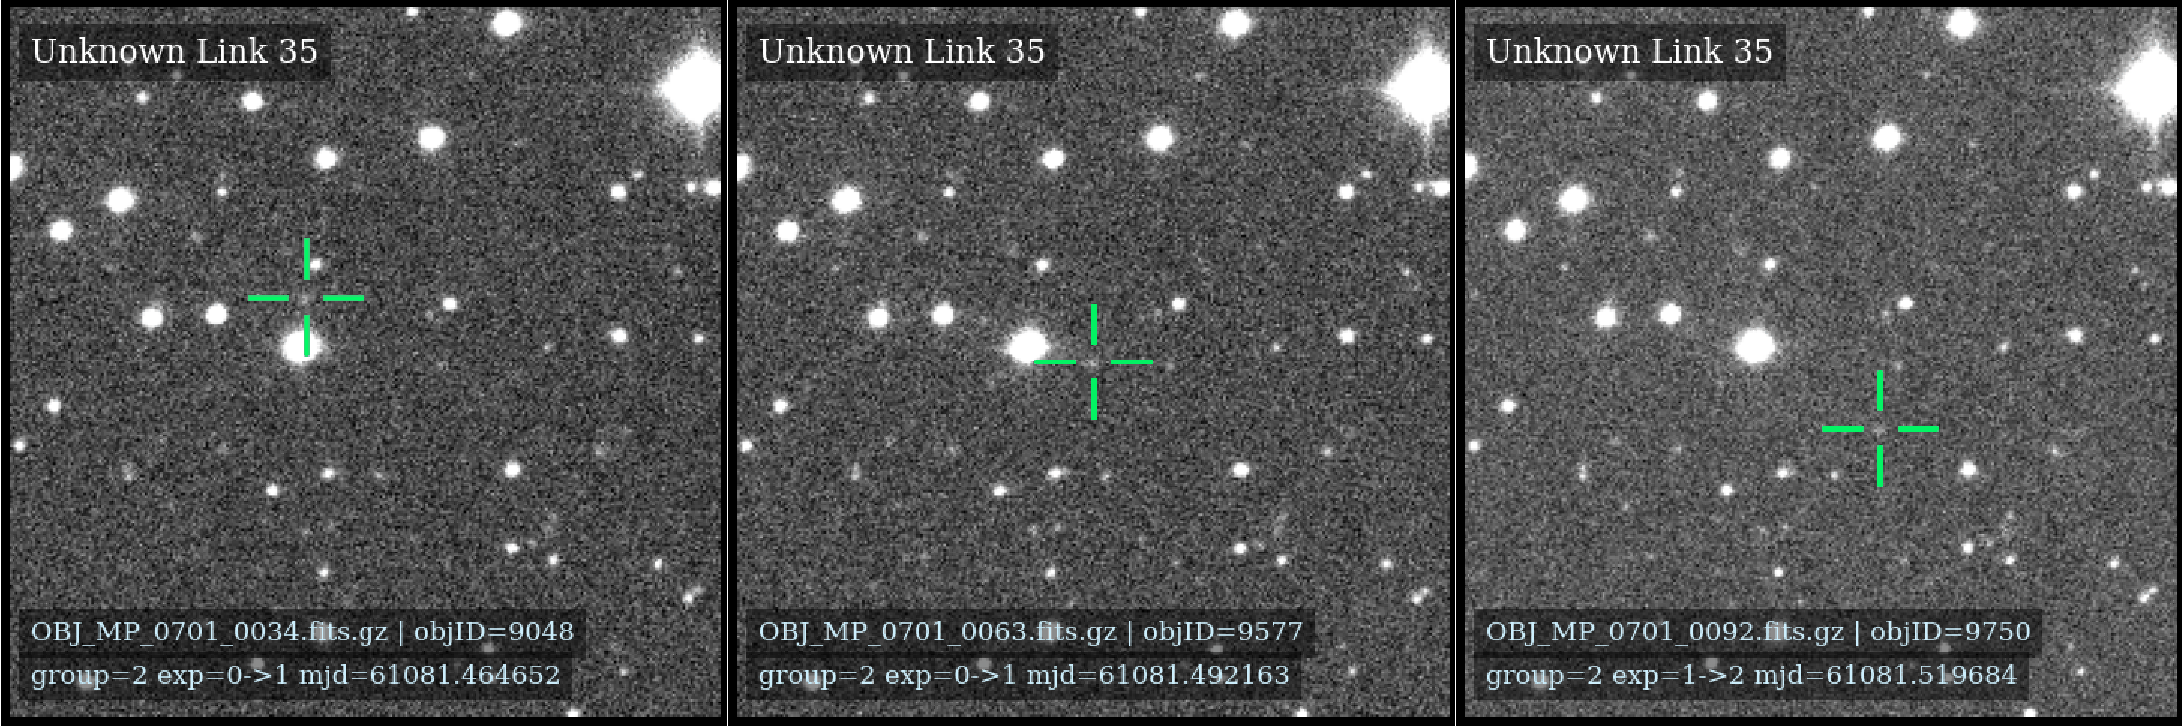
\includegraphics[width=\linewidth]{fig08_candidate.pdf}
\caption{The three original frames of the retained
2026 February~10 linkage 35, with historical
identifier \texttt{00000P2}. The panels are ordered
from left to right at UTC exposure midpoints
11:09:05.959, 11:48:42.908, and 12:28:20.720.
The green marker identifies the detection in each
frame. The fitted linear rate is approximately
61.34~\rateunit. This sequence is an example
of an image-reviewed single-night linkage.}
\label{fig:candidate}
\end{figure}

Two sets of archived ephemeris comparisons support
the numerical association of six retained links
with C/2025~Y1 (ATLAS). The comet remained in the
candidate stream because the contemporaneous
known-object prediction catalog contained asteroid
orbits. The other 52 links have unresolved
identities at the frozen analysis epoch. Their
measured positions, times, brightnesses, and
angular motion are the observational result;
authoritative identity reconciliation and
cross-night association would establish how
many physical objects they represent.
